\documentclass{beamer}

\usepackage[english, ngerman]{babel}	% Englische und deutsche Rechtschreibung
\usepackage[utf8]{inputenc}				% Umlaute-Darstellung unter Linux

\usecolortheme[]{default}

%-------------------- Titelblattinformationen ----------------------------
\title{Qualitätssicherung in einer Scrum basierten Entwicklungsumgebung}
\subtitle{Kurzvortrag}
\author{David Liebemann, Lucas Küntzer, Tobias Meier}
\institute{Fachhochschule Trier}
%--------------------------------------------------------------------------

\begin{document}

\begin{frame}
%------------------------- Titelblatt -------------------------------------
\titlepage
%--------------------------------------------------------------------------
\end{frame}

\begin{frame}
%----------------------- Scrum allgemein ----------------------------------
\frametitle{Scrum - Schritte}
\only<1>{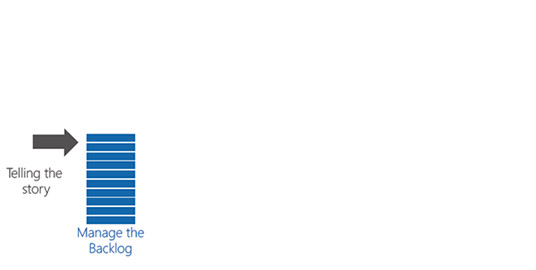
\includegraphics[scale=0.6]{./presGraphics/scrum01}}
\only<2>{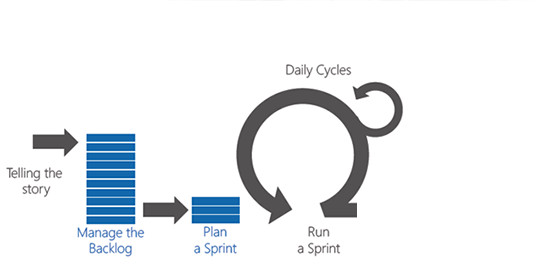
\includegraphics[scale=0.6]{./presGraphics/scrum02}}
\only<3>{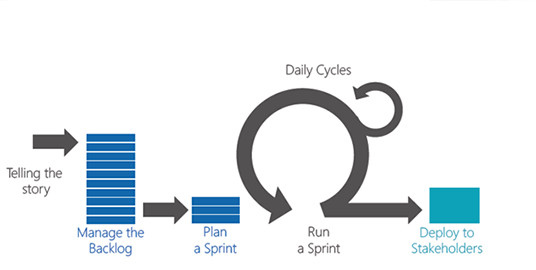
\includegraphics[scale=0.6]{./presGraphics/scrum03}}
\only<4>{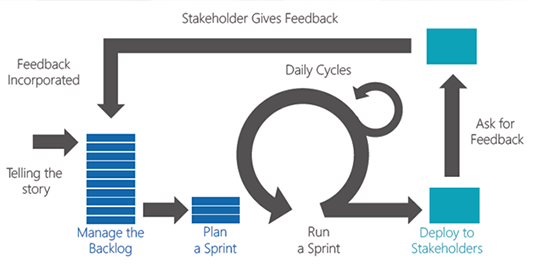
\includegraphics[scale=0.6]{./presGraphics/scrum}}
%--------------------------------------------------------------------------
\end{frame}

\begin{frame}
%-------------------- Wo muss QA betrieben werden ?------------------------
\frametitle{QA ja, aber wo?}
\begin{block}<1->{\color<4->{red}{nach dem Sprint}}
	\invisible<-2>{
		nicht Möglich da: 
		\begin{itemize}
			\item nach einem Sprint ein fertiges Inkrement vorhanden sein muss
		\end{itemize}
	}
\end{block}

\begin{block}<2->{\color<6->{green}{Wärend des Sprintes}}
	\invisible<-4>{
		nach den Regeln von Scrum möglich
	}
\end{block}
\only<5>{}	% damit gestoppt wird bevor es zur nächsten Folie geht
%--------------------------------------------------------------------------
\end{frame}

\begin{frame}
%---------------------- Ansprüche an das Testen ---------------------------
\frametitle{Ansprüche an das Testen}
\begin{itemize}
	\item schnelles Testen
	\begin{itemize}
		\item automatisiert
	\end{itemize}
\end{itemize}
%--------------------------------------------------------------------------
\end{frame}

\begin{frame}
%---------------- Beispiel von Testen in einem Sprint ---------------------
\frametitle{QA in einem Sprint}
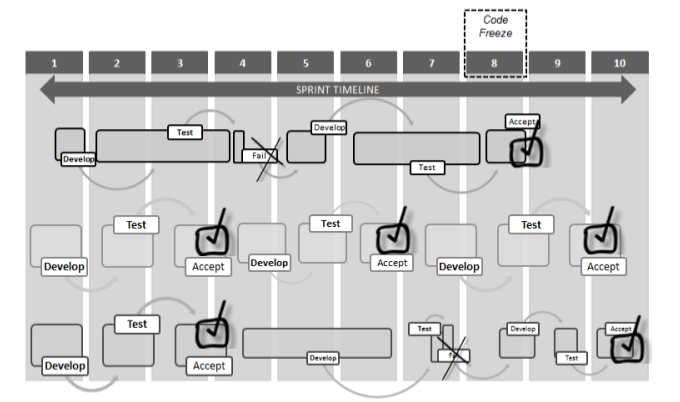
\includegraphics[scale=0.6]{./presGraphics/sprintQA}
%--------------------------------------------------------------------------
\end{frame}

\end{document}